
\chapter{Setup and technique details and instructions}\label{app:instructions}


The following procedures assume that the setup, hardware configuration, and Software interfaces have not changed since the publishing of this Thesis.

\section{Sniffer setup at DTU}\label{app:sniffer}


\begin{figure}[h!]
	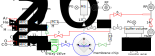
\includegraphics[width=\textwidth]{02_Tools/fig/setup_sniffer.png}
	\caption{Valve diagram of EC-MS setup at DTU. Adapted from Paper \ref{Trimarco2018}. Red: components installed since that publication. Green: The 6-way valve was removed since then as well as the pneumatic valves before the pressure controllers, which were re-purposed. Blue: The interface block, as well as the valve right before it, were replaced to minimize the intervening volume, enabling faster exchange of gases.}
	\label{fig:sniffer}
\end{figure}
Figure \ref{fig:sniffer} shows a valve diagram of the sniffer setup. Most of this setup was built during Daniel Trimarco's PhD project\cite{Trimarco2017_PhD}, and described in Paper \ref{Trimarco2018}. Colors indicate the parts that I have removed (green) or added (red) since Paper \ref{Trimarco2018}'s publication.

On the left of the diagram are mass flow controllers (MFC's) which can be used to switch between up to four gases at time. Switching between gases sharing an MFC, f.eks. Ar and He, requires pumping down behind the MFC through a line not shown. Moving right, we refer to the volume between Valves 7, 8, 9, 10, 11, and 12 and PC 1 as the \textit{gas manifold}. The gas manifold can be evacuated through Valve 7 and filled up from one of the MFC's while regulating the pressure with a pressure controller (PC), PC1.

Carrier gas from the gas manifold enters the interface block via Valve 8. The interface block guides it through the carrier gas reservoir channel of the chip, from which it fills the chip's sampling volume and saturates the electrochemical environment. Fast carrier gas exchange thus requires that the volume between valve 8 and the chip, the \textit{carrier gas inlet volume} is as small as possible. This is because the carrier gas inlet volume, unlike the gas manifold, cannot be pumped down, as the resulting vacuum in the sampling volume of the chip would suck in electrolyte. The design of the carrier gas inlet volume can also be optimized with regards to flow patterns to minimize mixing of the old and new carrier gas. 

We refer to the volume between PC1, PC2, and Valves 1, 5, 6, and 7 as the \textit{pumping manifold}. There are actually three possible ways to pump on the pumping manifold: (1) Directly to the \textit{roughing pump} (RP) through Valve 6, or (2-3) through a buffer volume and then a \textit{turbo molecular pump} (TMP or just turbo pump) via either a (2) valve 2 and a needle valve or (3) a gate valve. 
%Of these options, the direct roughing pump connection is the only one that can quickly remove a large amount of gas, as this would damage the turbo pump. Valve 14 should be closed while gas is fed directly to the roughing pump, as the pressure behind the turbo pump must also be kept low during operation. On the other hand, the turbo pump is required to reach high vacuum, which it can do slowly for a moderate amount of gas through the needle valve or quickly for a small amount of gas through the gate valve.

During operation, carrier gas is flowing from the gas manifold to the pumping manifold through the chip, and its pressure is regulated by PC2, which is set to 1 bar for all of the experiments in this Thesis. Excess carrier gas flows through PC2 to the pumping manifold where it is ultimately removed through the roughing pump, typically via the buffer volume and needle valve, so that valve 14 can remain open.

When a new chip is installed, the \textit{post-capillary volume} bound by the chip, Valve 13, and Valve 5 is vented to atmospheric pressure, and must be pumped down to high vacuum before connecting the experiment to the mass spectrometer. The mass spectrometer is always held at high vacuum by its own designated turbo and roughing pumps. The mass spectrometer of the sniffer setup is a Pfeiffer QMA125.

The procedures for chip pump-down and carrier gas exchange are described below.

An unusual feature of the sniffer setup, as mentioned in that Section, is that there are three ways to pump on the pumping manifold. Of these options, the direct roughing pump connection is the only one that can quickly remove a large amount of gas, as this would damage the turbo pump. Valve 14 should be closed while gas is fed directly to the roughing pump, as the pressure behind the turbo pump must also be kept low during operation. On the other hand, the turbo pump is required to reach high vacuum, which it can do slowly for a moderate amount of gas through the needle valve or quickly for a small amount of gas through the gate valve.

\subsection{Changing chip}
The procedure on this setup to change a chip is as follows:
\begin{enumerate}
	\item Isolate the chip: Make sure that Valves 13, 5, and 8 are closed, that no carrier gas is flowing, and that PC2 is closed (set to 2 bar). Double-check that Valve 13 is closed!!!
	
	\item Remove the old chip and put on the new chip.
	
	\item Close valves 1 and 14 and open valve 6 to connect the pumping manifold to the roughing pump. (The gate valve should be closed.)
	
	\item Open valve 5. This very quickly removes the majority of the gas from the post-capillary volume
	
	\item Close valve 6 and open Valve 1. Open valve 14.  
	
	\item Check the pressure displayed on the pressure guage (PG) of the buffer volume. The pressure in the buffer volume should already be less than 1 mbar. If not, the chip has not been installed correctly. If so, close valves 1 and 5 and start over.
	
	\item If the pressure in the buffer volume is greater than 0.3 mbar, start pumping through the needle by opening Valve 2.
	
	\item When the pressure in the buffer volume is less than 0.3 mbar (as will usually be the case right away after first roughing on the pumping manifold), open the gate valve. This is done by first deactivating 4 and then activating 3.
	
	\item When the pressure in the buffer volume is less than 0.0001 mbar, we can open to the mass spectrometer. Make sure that Valves 1 and 5 are open (so that the pressure on the buffer volume is equal to the pressure in the post-capillary volume), and open Valve 13.
	
	\item Immediately close Valve 5. This avoids making any subsequent mistake in which carrier gas enters the mas spectrometer via the pumping manifold. Also, close the gate valve. This is done by first deactivating 3 and then activating 4.
\end{enumerate}


\subsection{Changing carrier gas}
The procedure on this setup to change carrier gases is as follows. We will use the example of changing from He to \ch{H2}. This is what is done in Figure \ref{fig:RHE_cal}.

\begin{enumerate}
	\item At first, He is flowing through MFC1 at 1 ml/min and continues through Valve 9, Valve 8, the chip, PC2 (set to 1 bar), Valves 1 and 2, the turbo pump, Valve 14, and the roughing pump.
	
	\item Close valve 8. There is a reservoir of He in the interface block which will continue to fill the sampling volume of the chip for some time. Thus, the electrochemistry experiment can continue and the electrode ``won't notice'' that anything is going on.
	
	\item Stop the He flow by setting the flow on MFC 1 to zero. Valve 9 will automatically close.
	
	\item Close Valves 1, 2, and 14. Open Valve 6.
	
	\item Open Valve 7. This evacuates the He from the gas manifold. 
	
	\item Flush once with \ch{H2}. This can be done by setting the flow on MFC 2 to -1, which will be interpreted as ``go to purge mode for 1 second''.
	
	\item Close Valve 7. 
	
	\item Fill up the gas manifold with \ch{H2}. This is most quickly done by using the purge function. The purge time required is different for each gas. If you are unsure, enter -0.5 in the MFC, see how the pressure measured by PC1 increases, and then scale up the purge time accordingly. When the pressure is close to 1 bar, use normal flow (positive number for the MFC) to fill it up the rest of the way.
	
	\item If you overfill the gas manifold, such that the pressure read at PC 1 is significantly greater than 1 bar, this should be corrected, as a pressure difference when Valve 8 is opened seems to cause more mixing in the carrier gas inlet volume. Use PC1 to lower the pressure to 1 bar.
	
	\item When the pressure in the gas manifold is 1 bar: open Valve 8 and immediately set the MFC to its maximum flow value (10 ml/min for most MFC's). The change of carrier gas should be immediately apparent in the mass spectrometer signals.
	
	\item When the He level has dropped to background level (or by three orders of magnitude), lower the \ch{H2} flow rate to 1 ml/min. Note that the remaining He signal likely comes more from He dissolved in the elctrolyte in the outer volumes of the cell, and not necessarily the carrier gas. If so, the rate at which the remaining He signal continues to drop should not depend on the carrier gas flow rate.
	
	\item Close Valve 6, and open Valves 1, 2, and 14. The setup is now in steady operation in the new carrier gas.
	
\end{enumerate}


\section{ECMS-200A at CAS in Fuzhou}\label{app:Fuzhou}

\begin{figure}[h!]
	\centering
	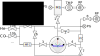
\includegraphics[width=0.75\textwidth]{02_Tools/fig/setup_Fuzhou.png}
	\caption{Valve diagram of EC-MS setup at Fuzhou. In reality, at the time of writing this thesis, the pressure controller is actually a modified pressure regulator, which works but is not as stable.}
	\label{fig:Fuzhou}
\end{figure}

The sniffer setup described above can be considered a ``delux setup'' with an excess of components to maximize functionality. The group in Fuzhou asked me to design a ``budget setup'' which captured the central advantages of chip EC-MS with as few components as possible. They then built my design, shown in Figure \ref{fig:Fuzhou} with the outside help from a Chinese mass spectrometer company, Quantang Instruments. Much to my frustruation, Quantang built a box around the valve system, making it quite tedious to make changes to the system, and put their logo and the name ECMS200A on the box.

All of the concepts are the same as for the sniffer setup, but the operation is different. The procedures for chip pump-down and carrier gas exchange are described in Appendix \ref{app:Fuzhou}. The cost of having one less Turbo pump is the need to wait for long pumping periods and to turn off the filament of the mass spectrometer when changing chips. The carrier gas exchange procedure is actually slightly simpler than that of the sniffer setup and saves three MFC's and a PC. The only disadvantage is that, with only one MFC, it is not easy to prepare a controlled gas mixture (a functionality I have rarely used on the sniffer setup).

\subsection{Changing chip}
The procedure to change chip is as follows:
\begin{enumerate}
	\item Isolate the chip: Close Valves 1, 2, 3, and 4. Double-check that Valve 1 is closed!!! Also, turn off the filament of the mass spectrometer
	
	\item Remove the old chip and install the new one.
	
	\item Open valve 2 (Valve 8 is normally always open). This removes air from the post-capillary volume through the roughing pump.
	
	\item Wait until the pressure is less than 0.01 mbar (1 Pa, the unit on the Chinese displays). This takes approximately half an hour.
	
	\item Double check that the filament of the mass spectrometer is turned off, as the roughing pressure could damage it. Then open Valve 1. 
	
	\item Immediately close Valve 2.
	
	\item When the pressure in the mass spectrometer is less than $10^{-5}$ mbar ($10^{-3}$ Pa), turn on the filament again. After this, it will take a couple hours before the MS signals are stable.	
\end{enumerate}



\subsection{Changing carrier gas}
The procedure for changing carrier gases (with He to CO as an example) is as follows:
\begin{enumerate}
	\item At first, He is flowing through Valve 10a, the MFC (set to 1 ml/min), Valve 3, the chip, Valve 4, the pressure controller set to 1 bar (actually a pressure regulator, adjusted to maintain 0 vs atmosphere), Valve 8 and the RP. 
	
	\item Close Valves 3 and 4. The electrochemistry experiment can then continue in He while getting the new carrier gas ready.
	
	\item Close Valve 10a and set the MFC to zero.
	
	\item Pump out the He. This involves opening Valves 5, 6, and 7, and setting PC to zero.
	
	\item Close Valves 5 and 6 and set PC to 1 bar.
	
	\item Fill up CO: Open Valve 10b. Then set the MFC to 10 ml/min. flow until the pressure read at PC is 1 bar.
	
	\item Close Valve 7 and open Valves 3 and 4. The carrier gas change should immediately be visible 
	
	\item Set the CO flow to 1 ml/min. The setup is now in steady operation in CO carrier gas.
\end{enumerate}



\section{Spectro Inlets}\label{app:spectro}

\begin{figure}[h!]
	\centering
	\includegraphics[width=0.75\textwidth]{02_Tools/fig/spectro.png}
	\caption{Photos of the setup at Spectro Inlets ApS. From their website: \url{https://spectroinlets.com/}}
	\label{fig:spectro}
\end{figure}
Finally, I should mention that there is now a commercially available setup which combines the best of both worlds: The functionality of the Sniffer setup and the simplicity and compactness of the ECMS200A. This is made possible in part due to some custom vacuum components. The setup, sold by Spectro Inlets ApS, is shown in the photographs in Figure \ref{fig:spectro}. I have been involved in conversations aiding the development of this setup, as a kind of test user, but can't go to detail here on its design. The Spectro Inlets setup also comes with a software automating the chip pump-down and carrier gas exchange procedures. The procedures described in Appendix \ref{app:instructions} for the other two setups are thus simplified to pressing a button.



\section{Sputtering \ch{Ru^{18}O2} and \ch{Ir^{18}O2}}\label{app:sputter}

This appendix serves as the sample prep methods for most of Chapter \ref{ch:O2}, as well as instructions for sputter deposition using \ch{^{18}O2}.

\subsection{Switching \ch{O2} source}
First, prepare the reactant gas. This requires a pump-down step to avoid mixing the natural \ch{O2} and the 99\% \ch{^{18}O2}.
\begin{enumerate}
	\item Make sure the flow is off (AJA software) and the reactant gas valve on the top of the sputter chamber (manually controlled) is open!
	
	\item Make sure both the natural oxygen (\ch{^{16}O2}) and \ch{^{18}O2} valves nearest the switch (the T intersection just before the flow controller) are closed.
	
	\item Evacuate the switch through the sputter chamber. This is a bit tedious because the AJA software will try to close the pneumatic valve when the flow doesn't reach set point. First flow at 10 ml/min until there is so little gas that this flow rate cannot be met. Then set it to 0.5 ml/min and leave it for an hour. The AJA software seems to have a tolerance of 0.5 ml/min before automatically closing the valves, so this will leave it open.
	
	\item Turn off the flow with the AJA software.
	
	\item Open the valve connecting the desired \ch{O2} source to the switch. 
	
	\item If you are using \ch{^{18}O2}, briefly open the valve on the bottle and close it again. The \ch{^{18}O2} in the line should then be enough for depositing a film, and this will avoid making a mistake that would waste the remaining gas.
\end{enumerate}

\subsection{Deposition}
The sputter deposition  process for nominally 25 (10) nm of \ch{Ru^{18}O2} (\ch{Ir^{18}O2}) is as follows:
\begin{enumerate}
	\item Load the samples via the load lock, and heat the samples to the desired temperature. 400$^\circ$C gives crystalline, rutile films.
	
	\item Pre-clean the chamber with an argon plasma for 5 minutes. Use 20 ml/min Ar, 20 mTorr, and 35 Watts.
	
	\item Put the screen in front of the samples. Sputter titanium. Use 20 ml/min Ar, 3 mTorr, and 160 W. You may need to start the plasma at 10 mTorr and then ramp down. This step is to remove any residual oxygen in the chamber to achieve isotopic purity. (This step can be skipped when not doing isotope-labeled films.)
	
	\item After titanium has been sputtering for 15 minutes, remove the screen and allow it to keep sputtering, now onto the samples, for another three minutes. This establishes a $\approx$ 5 nm thick Ti sticking layer. After three minutes, close the shutter again and keep sputtering Ti for another three minutes before turning off the Ti plasma.
	
	\item Increase the pressure to 5 mTorr and lower the Ar flow rate to 5 ml/min. 
	
	\item Start the plasma on the Ru (Ir) target. Use 60 W (30 W).
	
	\item Start the \ch{^{18}O2} flow at 1 ml/min.
	
	\item Open the shutter to the Ru (Ir) target. 
	
	\item Time 1500 s (700 s), and then close the shutter
	
	\item Turn off the plasma.
	
	\item Turn off the gas flows.
	
	\item Let the samples cool before taking them out through the load lock.
\end{enumerate}


\section{ICP-MS}\label{app:sampling}


Briefly, the electrolyte in the cell is sucked out with a syringe while new electrolyte flows in from an electrolyte delivery tower. The old electrolyte stored in an Eppendorf tube and the syringe is re-inserted. This results in electrolyte samples of $\approx 0.5$ ml in Eppendorf tubes. 

For study with ICP-MS, the raw samples are first diluted to a standard volume of 1 ml with 2\% \ch{HNO3}, 0.1 ml of this is then diluted to 10 ml with 2\% \ch{HNO3}, which is the ICP-MS sample. The concentration of this ICP-MS sample is then as if all of the metal dissolved during the experiment were diluted in 100 ml. The amount of metal $n^i$ (typically stated in pmol) can then be determined from its mass concentration $c_m^i$ in the ICP-MS sample (typically stated in $\mu$g per l which is numerically equivalent to ppb) by
\begin{equation}
n^i = 100\,\text{[ml]}\frac{c_m^i}{M^i}\,,\label{eq:ppb_to_pmol}
\end{equation}
where $M^i$ is the molar mass of $i$.

To determine $c_m^i$ from the raw signal (in counts) requires calibration. A dilution series (typically 0.1, 1, 10, and 100 $\mu$g/l) is prepared from a standard stock solution. These are measured together with the samples and intervening measurements a blank solution (2\% \ch{HNO3} in water with no metals). The calibration curve is made by drawing a line of best fit through the counts vs concentrations of this dilution series on a log-log plot (the slope of this line should be 1). Typical calibration curves for Ir and Ru are shown in Figure \ref{fig:ICPMS_cal}. These calibration curves are made using the function \texttt{ICPMS\_calibration} of the \texttt{EC\_MS} python package (see Appendix \ref{app:EC_MS}).

\begin{figure}[h!]
	\centering
	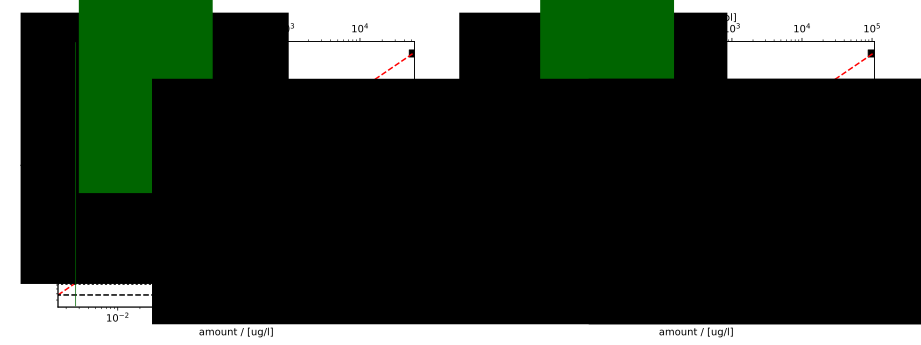
\includegraphics[width=\textwidth]{02_Tools/fig/ICPMS_calibration_curves.png}
	\caption{Calibration curves for ICP-MS detection of \textbf{(a)} Ir and \textbf{(b)} Ru. The top x-axes represents the amount of metal originally in a sample from the EC-MS setup, and is scaled to the bottom x-axis according to Equation \ref{eq:ppb_to_pmol}. The dashed black line is the mean number of counts in blank measurements, and the dotted black line is that mean plus three times the standard deviation of the number of counts in the blank measurement. The detection limit, defined as where the latter intercepts the calibration curve, is indicated with a green vertical line.}
	\label{fig:ICPMS_cal}
\end{figure}

The detection limit is defined as the amount corresponding to the counts of the blank measurements plus three times the standard deviation of counts the blank measurements\cite{Harris2010}. This is 1.4 pmol for Ir and 3.1 pmol for Ru.


\subsection{Electrolyte sampling}
It is possible with the sniffer setup to take electrolyte samples out under potential control for analysis with ICP-MS. This requires an electrolyte delivery bottle on one side and a syringe on the other side, as shown in Figure \ref{fig:ICPMS} on Page \pageref{fig:ICPMS}. To set this up (items 1 through 4 are the standard procedure):
\begin{enumerate}
	\item Align the sample in the cell
	
	\item Mount the cell on the interface block
	
	\item Fill the cell with electrolyte using the syringe
	
	\item Insert the RE and CE glassware when the electrolyte forms a miniscus in the Luer fitting
	
	\item When there is a miniscus of electrolyte coming out of the outlet (male Luer fitting), very quickly open the valve on the electrolyte delivery tower and push the tube onto the Luer fitting, connecting the tower and the cell. This should be done quickly to minimize spilling. Clean up any spill right a way with a paper wipe.
	
	\item Close the valve.
\end{enumerate}

It is important that valve is open while the electrolyte delivery tower is connected the cell to avoid developing an overpressure which could breach the chip. It is good for it to be closed during the experiment, or the pressure of the electrolyte above the valve can push electrolyte into the cell and exascerbate any leaks that might be present.

To take an electrolyte sample:
\begin{enumerate}
	\item Open the valve to the electrolyte delivery tower
	
	\item Pull 0.5 ml of electrolyte with the syringe. Do so as steadily as possible to avoid making an underpressure which could pull carrier gas from the chip into the working volume. Bubbles are the enemy!
	
	\item Remove the syringe and close the valve of the electrolyte delivery tower as fast as possible to minimize spillage. Clean up any spillage.
	
	\item Empty the syringe into an eppendorf tube or other storage. This is your sample for ICP-MS.
	
	\item Very quickly open the valve to the electrolyte delivery tower and quickly re-insert the syringe.
	
	\item Close the valve. You're ready to take the next sample when the time comes.
\end{enumerate}

